\documentclass[a4paper]{article}

\usepackage[francais]{babel}
\usepackage{xltxtra,fontspec,xunicode}

\usepackage{listings}

\usepackage{graphicx}
\usepackage{float}


\usepackage{listings}
\lstset{                                                                          
   basicstyle=\ttfamily,                                                           
   frame=lrtb ,
   columns=fullflexible      
}

\begin{document}
\section{Introduction}
Le but de ce project et de réaliser une application de tracking GPS, qui 
permet à un ensemble d'utilisateurs de partager leur trajets en temps réel.

\begin{figure}[H]
  \begin{center}
  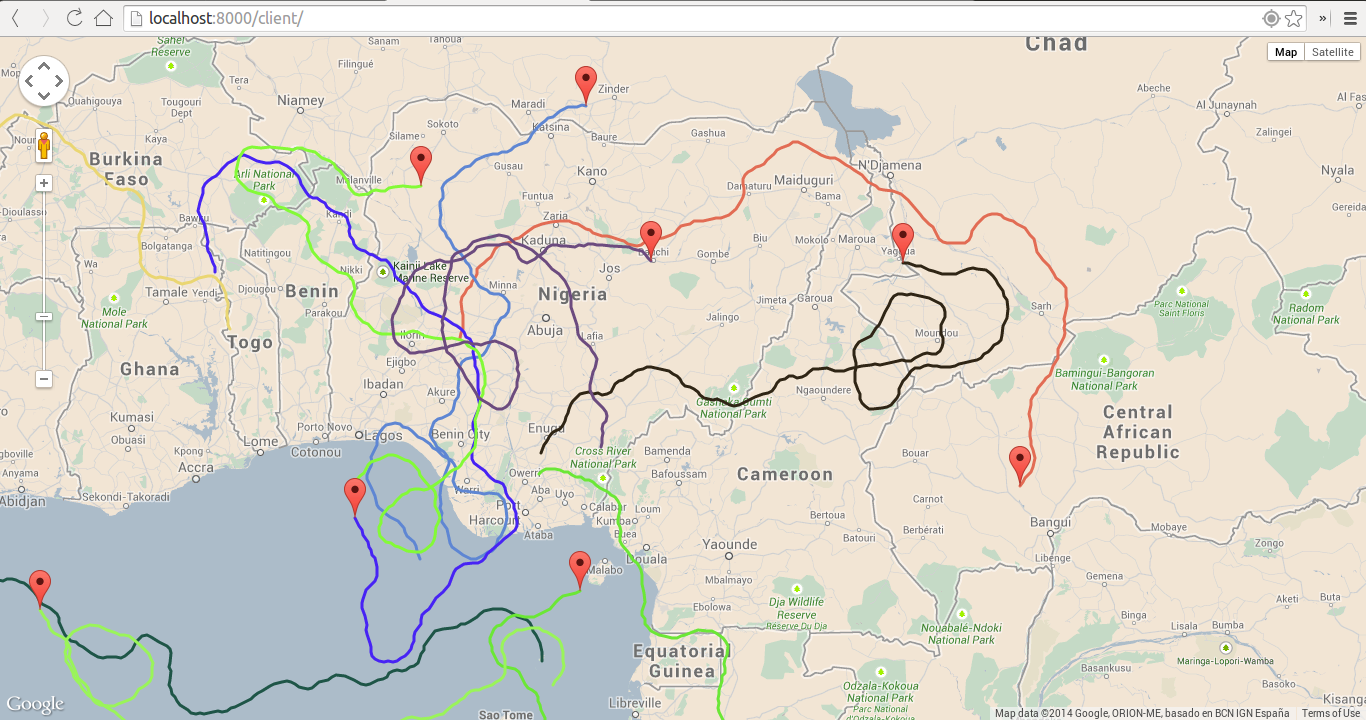
\includegraphics[scale=0.25]{screenshot.png}
  \end{center}
\end{figure}

Afin de réliser cette application nous avons utilisé les outils suivants :

\section{Outils utilisés}
\subsection{Node.js}

\begin{figure}[H]
  \begin{center}
  
\includegraphics[scale=0.5]{nodejs.png}
  \end{center}
\end{figure}

Node.js est une plateforme logicielle libre et événementielle en 
JavaScript orientée vers les applications réseau.

Elle utilise la machine virtuelle V8 et implémente sous 
licence MIT les spécifications CommonJS. 

Node.js contient une bibliothèque de 
serveur HTTP intégrée, ce qui rend possible de faire tourner un serveur 
web sans avoir besoin d'un logiciel externe comme Apache ou Lighttpd, 
et permettant de mieux contrôler la façon dont le serveur web fonctionne.

\subsection{Socket.io}

\begin{figure}[H]
  \begin{center}
  
\includegraphics[scale=1]{socketio.png}
  \end{center}
\end{figure}

Socket.io est un framework pour les application temps-réel. Il est composé de deux 
partie: une partie client qui tourne sur un navigateur et une autre serveur qui tourne sur Node.js.
Le deux parties ont une API identique.

La technologie principale que Socket.io utilise est le protocol WebSockets, mais il
peut utiliser d'autres méthodes comme Flash, Long-polling, ou JSONP.

\subsection{Angular.js}

\begin{figure}[H]
  \begin{center}
  
\includegraphics[scale=1]{angularjs.png}
  \end{center}
\end{figure}

Angular.js est un framework Javascript coté-client dévélopé par Google
qui à pour but d'accélerer le développement d'applications web monopages.
Il propose d'étendre la syntax de HTML avec des balises personnlisées, organiser 
l'application sous une architecture MVC, communiquer avec le serveur, routing, 
data-binding et autres fonctionnalités.

\subsection{Phantom.js et Casper.js}

\begin{figure}[H]
  \begin{center}
  
\includegraphics[scale=0.5]{phantomjs.png}
  
\includegraphics[scale=0.2]{casperjs.png}
  \end{center}
\end{figure}

Phantom.js et un `headless browser' c'est à dire un navigateur sans interface
graphique mais qui a API qui permet d'écrire des tests pour les applications
web coté client.

Casper.js est un framework de Phantom.js qui facilite l'écriture de ces scripts.

\section{Réalisation}

\subsection{Serveur HTTP}

Le code suivant utilise le framework express pour servir les fichier html, css et Javascript
qui se trouve dans le dossier client
et lance le serveur HTTP sur le port `port' : 

\begin{lstlisting}
var express = require('express')
  , http = require('http');

// create http server
var app = express()
  , server = http.Server(app);

// serve client's static files
app.use('/client', express.static(__dirname + '/../client'));

// run the server
var port = process.argv[2] || 8000;
server.listen(port, function() {
  console.log('Server started : http://localhost:' 
  + port + '/client');
});
\end{lstlisting}

\subsection{Transmition de données en temps réel}


\subsubsection{Le modèle:}

On déclare une classe Users qui contient la liste des utilisateurs
et leurs données géographiques.

\begin{lstlisting}
function Users() {
  this._users = {}; // the list of users
}
\end{lstlisting}

On ajoute des méthodes qui manipulent la liste \_users tout en envoyant des signaux
vers les clients pour les prévenir des changements de données\\

\textbf{Ajout d'un utilisateur : }

\begin{lstlisting}
Users.prototype.addUser = function(socket) {
  this._users[socket.id] = [];

  // tell all other users
  socket.broadcast.emit('add user', socket.id);

  // send the list of users to the new one
  socket.emit('list', this._users);
};
\end{lstlisting}

\textbf{Suppression d'un utilisateur : }
\begin{lstlisting}
Users.prototype.removeUser = function(socket) {
  delete this._users[socket.id];

  // inform other users
  socket.broadcast.emit('remove user', socket.id);
}
\end{lstlisting}

\textbf{Ajout d'un mouvement de l'utilisateur:}
\begin{lstlisting}
Users.prototype.addStep = function(socket, pos) {
  this._users[socket.id].push(pos);

  // tell everyone else this user moved 
  socket.broadcast.emit('add step', {id: socket.id, pos : pos});
}
\end{lstlisting}

\subsubsection{Le controlleur:}

Dans le controlleur on répond au signux de l'utilsateur et on manipule 
le modèle.

\begin{lstlisting}
 var socketio = require('socket.io')
   , Users = require('../models/users');

 // start socket.io
 var io = socketio.listen(server)
   , users = new Users();

 // The user connects
 io.sockets.on('connection', function(socket) {
    users.addUser(socket);
    
    // he moves
    socket.on('moved', function(pos) {
      users.addStep(socket, pos);
    });

    // or quits
    socket.on('disconnect', function() {
      users.removeUser(socket);
    });
 });
\end{lstlisting}

\subsection{Le Client}

Le client est écrit en utilisant Angular.js et le module angular-google-maps
ce dernier permet d'utiliser l'API Google maps avec des directives.

\subsubsection{Les modèles}

\textbf{Options Google maps : }
\begin{lstlisting}
  var app = angular.module('gps-tracking');

  app.value('map', {
    center: {
      latitude: 0,
      longitude: 0
    },
    zoom: 8
    // ...
  });
\end{lstlisting}
\textbf{Liste des utilisateurs}

\begin{lstlisting}
  // socket.io
  app.factory('socket', function() {
    return io.connect('/');
  });

  // users' positions
  app.value('users', {});
\end{lstlisting}

\subsubsection{Le controlleur}

Dans le controlleur on répond aux signaux du serveur qui sont : 

\begin{itemize}
  \item \textbf{list} : Envoie la liste de tous les utilisateurs qui sont déja connéctés.
  \item \textbf{add user} : Ajout d'un nouvel uilisateur.
  \item \textbf{remove user} : Suppression d'un utilisateur.
\end{itemize}

Ensuite on apelle watchPosition qui nous permet de mettre à jour les coordonées de l'utilisateur.

\begin{lstlisting}

app.controller('MapController', function (
   $scope, map, socket, users, helpers, STROKE_WIDTH) {
  // THE LIST OF USERS
  $scope.users = users;

  // GOOGLE MAPS SETTINGS
  $scope.map = map;

  // SOCKET.IO SERVER
  socket.on('list', function(list) {
    $scope.$apply(function() {
      // Add previousely connected users
      for(var id in list) {
        users[id] = {
          stroke : {
            color: helpers.getRandomColor(),
            stroke: STROKE_WIDTH
          },
          path: list[id]
        };
      }
    });
  });

  socket.on('add user', function(id) {
    $scope.$apply(function() {
      users[id] = {
        stroke : {
          color: helpers.getRandomColor(), 
          stroke: STROKE_WIDTH
        },
        path : []
      };
    });
  });

  socket.on('remove user', function(id) {
    $scope.$apply(function() {
      delete users[id];
    });
  });

  socket.on('add step', function(data) {
    $scope.$apply(function() {
      users[data.id].path.push(data.pos);
    });
  });

  // GEOLOCATION API
  navigator.geolocation.watchPosition(
    // Sucess callback
    function (pos) {
      var p = {
        timestamp: pos.timestamp, 
        longitude: pos.coords.longitude, 
        latitude:  pos.coords.latitude 
      };

      // send signal to the server and update local data
      if(!users[socket.id]) {
        users[socket.id] = {
          stroke: {
            color: helpers.getRandomColor(), 
            weight: STROKE_WIDTH
          },
          path: []
        };
      }
      
      // store locally
      users[socket.id].path.push(p);
      
      // send to server
      socket.emit('moved', p);
    },
    // Error callback
    function (err) { 
      alert(err.message);
    }
  );
});
\end{lstlisting}

\subsection{La vue}

A l'aide du module angualar-google-maps on peut afficher les données stockées dans le 
tableau users dans Google maps on utilisant les derictives suivantes:

\begin{lstlisting}

  <google-map center="map.center" zoom="map.zoom" 
    draggable="true" options="map.options">
      <polyline ng-repeat="user in users" path="user.path" 
        stroke="user.stroke">
      </polyline>
    <marker ng-repeat="user in users" 
      ng-show="user.path.length > 0" coords="user.path | last">
    </marker>
  </google-map>
\end{lstlisting}


\section{Testing}

Pour tester l'application avec un grand nombre de clients connecté en même temps.
On doit uttiliser Casper.js. Mais malheureusement ce dernier ne supporte pas
l'API geolocation donc on a construit un module qui permet d'ajouter cetter API, 
et de contrôler la position du client virtuel.

\begin{lstlisting}

/** casperjs-geolocation
  * A capser module that mocks the geolocation API
  */

// functions to be evaluated in remote
var Remote = {
  add_geolocation_api : function(pos) {
    navigator.geolocation = {
      // store pos here
      __casperFakeLocation : pos,
      
      // getcurrentposition
      getCurrentPosition : function(callback, err) {
        callback({coords : this.__casperFakeLocation});
      },

      // stores the callback passed to watchPosition
      __casperWatchCallback : undefined,

      // watchposition
      watchPosition : function(callback) {
        this.__casperWatchCallback = callback;
        console.log('watchPosition called');
        callback(this.__casperFakeLocation);
      }
    };
  },

  update_position : function(pos) {
    navigator.geolocation.__casperFakeLocation = pos;
    navigator.geolocation.__casperWatchCallback(pos);
  }
};

// module
var Geolocation = function(casper, pos) {
  this._pos = pos || {longitude : 0, latitude : 0};
  this._casper = casper;
};

Geolocation.prototype.getPos = function () {
  return this._pos
};

Geolocation.prototype.setPos = function(pos) {
  this._pos = pos;
  this._casper.evaluate(Remote.update_position, {
    timestamp: Date.now(),
    coords: {
      longitude: pos.longitude,
      latitude: pos.latitude
    }
  });
};

module.exports = function(casper, pos) {
  var geo = new Geolocation(casper, pos);
  casper.on('page.initialized', function() {
    geo._casper.evaluate(Remote.add_geolocation_api, pos);
  });
  return geo;
}
\end{lstlisting}

Ensuite on écrit le script qui lance un nombre (détérminer par des arguments CLI)
de clients qui changent leurs position géographique aléatoirement chaque second.
Et on regearde l'affichage des données dans l'application.

\begin{lstlisting}

/**
  * test.js
  * Test file that instanciate phantom.js clients
  * CLI argumetns : 
  *  --clients : number of clients
  *  --url : the url of the node.js server
  */
var require = patchRequire(require)
  , casperFactory = require('casper')
  , geoFactory = require('./casperjs-geolocation/'
        +'casperjs-geolocation.js');

try {
  var casper = casperFactory.create();
  // Display help  
  if(casper.cli.args[0] === 'help')
    throw new {name:'CLI', 
      message : 'casper test.js --clients=10' };

  // cli args
  var clientsCount = casper.cli.options.clients || 10
    , serverUrl = casper.cli.options.url 
        || 'http://localhost:8000/client';

  // Creating casper instances
  console.log('Creating ' + clientsCount + 'clients');
  var caspers = [];
  for (var i = 0; i < clientsCount; ++i) 
    caspers.push(casperFactory.create(
      {verbose:true, logLevel:'debug'}));

  // starting 
  caspers.forEach(function(casper) {

    // go to website
    casper.start(serverUrl);

    // Go to random geoposition
    var geo = geoFactory(casper, {
      longitude : Math.random() * 10,
      latitude : Math.random() * 10
    });

    // Change geolocatio every second
    var lats = []
      , lons = [];

    var x = Math.random() * 10
      , y = Math.random() * 10
      , angle = 0;

    casper.wait(1000, function changePosition() {

      angle = angle + 0.5 - Math.random() * 1;

      x1 = x + 0.1 * Math.cos(angle);
      y1 = y + 0.1 * Math.sin(angle);

      if (Math.abs(x1 - x) + Math.abs(y1 - y) < 10)
        geo.setPos({latitude: x1, longitude: y1});
      x = x1; y = y1;

      this.wait(1000, changePosition);
    });

    // display console.log() from remote
    casper.on('remote.message', function(msg) {
      this.echo('[remote] ' + msg, 'INFO');
    });

    // Run and wait
    casper.wait(9999999);
    casper.run();
  });

} catch (e) {
  if(e.name === 'CLI')
    console.log(e.message);
  else 
    throw e;
}
\end{lstlisting}
\end{document}


